\begin{center}
\underline{\Large{Losas de Escalera}}
\end{center}

\underline{Datos:}\\
Hormigón H-25 $\Rightarrow f'c = 250 \frac{Kg}{cm^2} = 25 MPa$\\
Acero ADN 42/50 $\Rightarrow fy = 4200 \frac{Kg}{cm^2} = 420 MPa$\\
Recubrimiento Cc = 2cm\\

\begin{figure}[H]
\begin{center}
     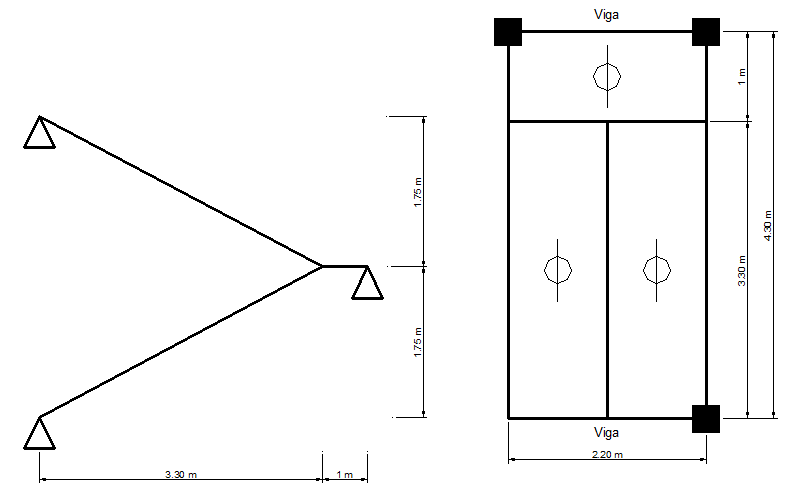
\includegraphics[scale = 0.85]{chapters/chapter_2/images/escalera1.png}
\end{center}
\end{figure}
\begin{figure}[H]
\begin{center}
     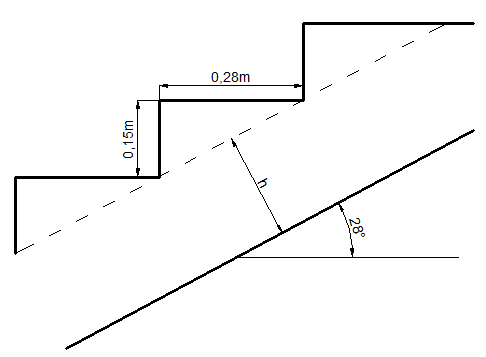
\includegraphics[scale = 0.8]{chapters/chapter_2/images/escalera2.png}
\end{center}
\end{figure}
\newpage
\begin{enumerate}
\item \underline{Predimensionado}
\begin{align*}
& h \geq = \frac{l}{20} = \frac{430cm}{20cm} = 21.3cm \quad \text{Adopto}\Rightarrow \framebox{$21cm$}
\end{align*}

\item \underline{Análisis de cargas}
\begin{align*}
& \text{Peso propio} \rightarrow 0.21m \cdot \frac{2500 \frac{Kg}{m^3}}{Cos(28\text{°})} = \framebox{$595 \frac{Kg}{m^2}$}\\
& \text{Peso propio escalones} \rightarrow \frac{0.15m}{2} \cdot 2200 \frac{Kg}{m^3} = \framebox{$165 \frac{Kg}{m^2}$}\\
& \text{Peso propio de carpeta} \rightarrow \frac{(0.282m + 0.15m)}{0.282m} \cdot 0.015m \cdot 2100 \frac{Kg}{m^3} = \framebox{$48 \frac{Kg}{m^2}$}\\
& \text{Peso propio de piso} \rightarrow \frac{(0.282m + 0.15m)}{0.282m} \cdot 0.012m \cdot 2800 \frac{Kg}{m^3} = \framebox{$51 \frac{Kg}{m^2}$}\\
& \text{Peso propio de cielorraso} \rightarrow 0.02m \cdot \frac{1200 \frac{Kg}{m^3}}{Cos(28\text{°})} = \framebox{$27 \frac{Kg}{m^2}$}\\
& D = \framebox{$886 \frac{Kg}{m^2}$}\\
& L = \framebox{$500 \frac{Kg}{m^2}$} \rightarrow \text{Según CIRSOC 101-05 - Capítulo 4}\\
& q_u = 1.2 \cdot D + 1.6 \cdot L = 1.2 \cdot 886 \frac{Kg}{m^2} + 1.6 \cdot 500 \frac{Kg}{m^2} = \framebox{$1863.2 \frac{Kg}{m^2}$}\\
& q_u = 1.4 \cdot D = 1.4 \cdot 886 \frac{Kg}{m^2} = \framebox{$1240.4 \frac{Kg}{m^2}$}
\end{align*}

\item \underline{Modelado en RAM}\\
Mediante software se modelo la estructura de escalera con dos sistemas de apoyo, cargando los valores de D y L para luego realizar las combinaciones de carga $1.2 \cdot D + 1.6 \cdot L$ y $1.4 \cdot D$\\
De la modelación por software se obtuvieron los momentos máximos positivos y negativos que se utilizarán para dimensionar las armaduras superior e inferior de las losas de escalera.\\
\begin{figure}[H]
\begin{center}
     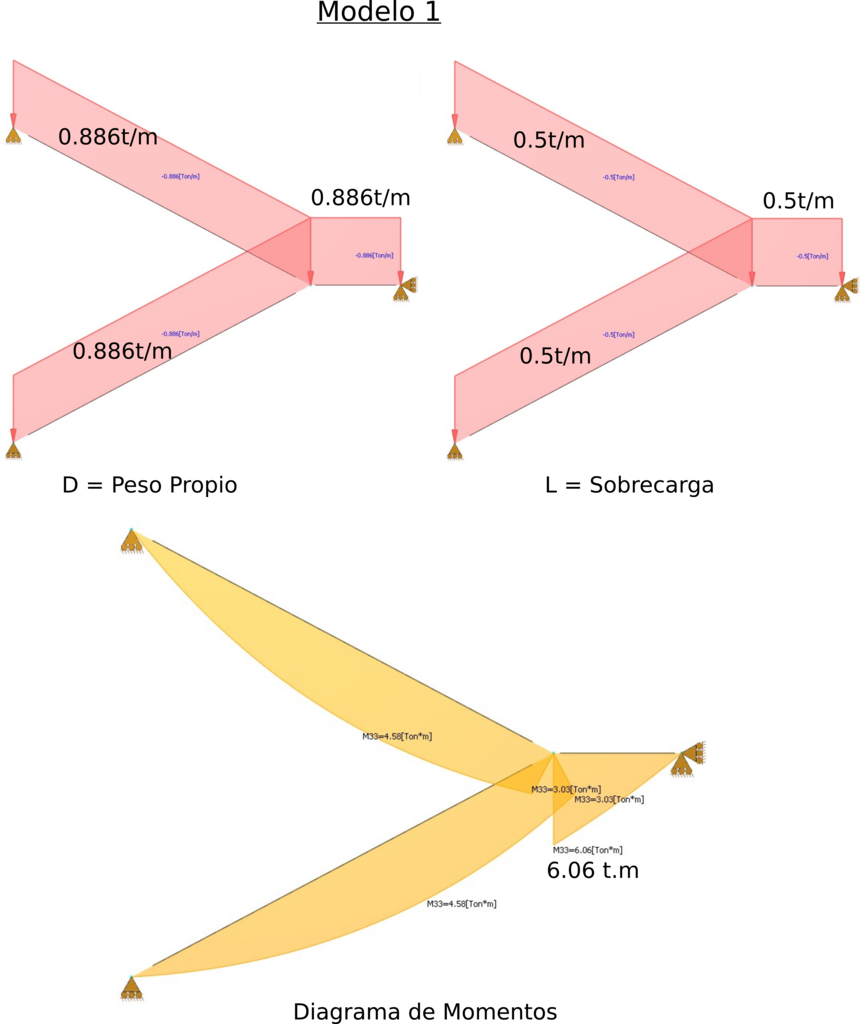
\includegraphics[scale = 4.2]{chapters/chapter_2/images/modelo1.png}
\end{center}
\end{figure}
\begin{figure}[H]
\begin{center}
     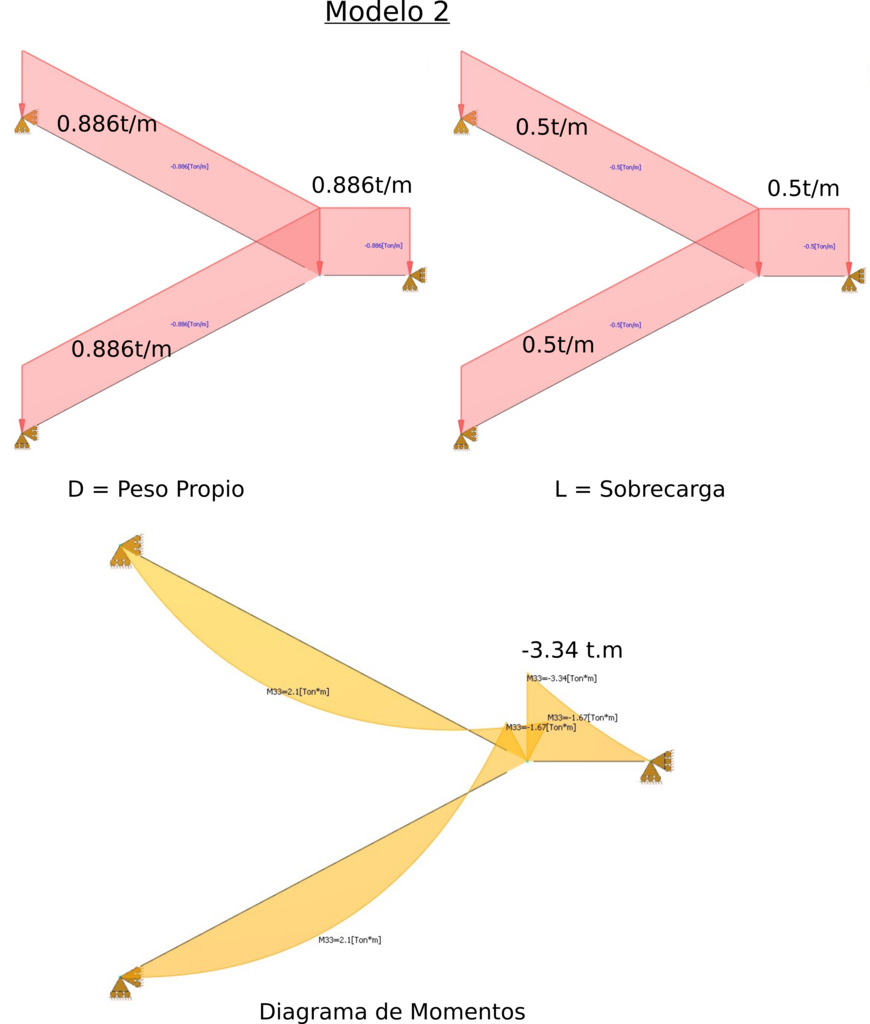
\includegraphics[scale = 4.2]{chapters/chapter_2/images/modelo2.png}
\end{center}
\end{figure}

\item \underline{Esfuerzos últimos}\\

\begin{align*}
& M_u = 6.06 \frac{t \cdot m}{m}\\
& M_u = -3.34 \frac{t \cdot m}{m}
\end{align*}
\newpage
\item \underline{Armadura Inferior}

\begin{align*}
& M_u = 6.06 \frac{t \cdot m}{m} \\
& M_n = \frac{M_u}{\phi} = \frac{6.06 \frac{t \cdot m}{m}}{0.9} = 6.73 \frac{t \cdot m}{m} \Rightarrow 0.067 \frac{MN \cdot m}{m} \\
& d = h -db - Cc - \frac{db}{2}= 21cm - 1.2cm - 2cm - \frac{1cm}{2}= 17.8cm \\
& Kd = \frac{d}{\sqrt[]{\frac{M_n}{b}}} = \frac{0.178m}{\sqrt[]{\frac{0.067 \frac{MN \cdot m}{m}}{1m}}} = 0.688 \Rightarrow Ke = 25.121 \\
& A_s = Ke \cdot \frac{M_n}{d} = 25.121 \cdot \frac{0.067 \frac{MN \cdot m}{m}}{0.178m} = 9.46 \frac{cm^2}{m}\\
& As_{min} = 0.0018 \cdot b \cdot h = 0.0018 \cdot 100cm \cdot 21cm = 3.78 \frac{cm^2}{m}
\end{align*}

Se adopta A° inferior $\phi$ 12 cada 12cm $\rightarrow \framebox{$9.48 \frac{cm^2}{m}$}$ \\

\underline{Verificación de separaciones}\\

\[ s = 12cm \leq \left\{ \begin{array}{ll}
         2.5 \cdot h = 2.5 \cdot 21cm = 52.5cm \quad \surd & \\
         25 \cdot db = 25 \cdot 1.2cm = 30cm \quad \surd &\\
         30cm \quad \surd & \end{array} \right. \] 
         
\[ s = 12cm \geq \left\{ \begin{array}{ll}
         db = 1.2cm \quad \surd & \\
         \geq 2.5cm \quad \surd &\\
         \geq \frac{4}{3} \cdot \text{Tamaño máximo del agregado} & \end{array} \right. \] 

\item \underline{Armadura Superior}

\begin{align*}
& M_u = 3.34 \frac{t \cdot m}{m} \\
& M_n = \frac{M_u}{\phi} = \frac{3.34 \frac{t \cdot m}{m}}{0.9} = 3.71 \frac{t \cdot m}{m} \Rightarrow 0.037 \frac{MN \cdot m}{m} \\
& d = h -db - Cc - \frac{db}{2}= 21cm - 1.2cm - 2cm - \frac{1cm}{2}= 17.8cm \\
& Kd = \frac{d}{\sqrt[]{\frac{M_n}{b}}} = \frac{0.178m}{\sqrt[]{\frac{0.037 \frac{MN \cdot m}{m}}{1m}}} = 0.925 \Rightarrow Ke = 24.583 \\
& A_s = Ke \cdot \frac{M_n}{d} = 24.583 \cdot \frac{0.037 \frac{MN \cdot m}{m}}{0.178m} = 5.11 \frac{cm^2}{m}\\
& As_{min} = 0.0018 \cdot b \cdot h = 0.0018 \cdot 100cm \cdot 21cm = 3.78 \frac{cm^2}{m}
\end{align*}

Se adopta A° superior $\phi$ 10 cada 15cm $\rightarrow \framebox{$5.24 \frac{cm^2}{m}$}$ \\

\underline{Verificación de separaciones}\\

\[ s = 15cm \leq \left\{ \begin{array}{ll}
         2.5 \cdot h = 2.5 \cdot 21cm = 52.5cm \quad \surd & \\
         25 \cdot db = 25 \cdot 1cm = 25cm \quad \surd &\\
         30cm \quad \surd & \end{array} \right. \] 
         
\[ s = 15cm \geq \left\{ \begin{array}{ll}
         db = 1cm \quad \surd & \\
         \geq 2.5cm \quad \surd &\\
         \geq \frac{4}{3} \cdot \text{Tamaño máximo del agregado} & \end{array} \right. \] 

\item \underline{Armadura Transversal de repartición}
\begin{align*}
& As_{min} = 0.0018 \cdot b \cdot h = 0.0018 \cdot 100cm \cdot 21cm = 3.78 \frac{cm^2}{m}
\end{align*}

Se adopta A° transversal de repartición $\phi$ 8 cada 12cm $\rightarrow \framebox{$4.19 \frac{cm^2}{m}$}$ inferiores\\

\underline{Verificación de separaciones}\\

\[ s = 12cm \leq \left\{ \begin{array}{ll}
         2.5 \cdot h = 2.5 \cdot 21cm = 52.5cm \quad \surd & \\
         25 \cdot db = 25 \cdot 0.8cm = 20cm \quad \surd &\\
         30cm \quad \surd & \end{array} \right. \] 
         
\[ s = 12cm \geq \left\{ \begin{array}{ll}
         db = 0.8cm \quad \surd & \\
         \geq 2.5cm \quad \surd &\\
         \geq \frac{4}{3} \cdot \text{Tamaño máximo del agregado} & \end{array} \right. \] 

\end{enumerate}